\section{Evaluation Setup}
\label{sec:eval-setup}
In this section, we describe the setup used in our evaluations. Our experimental environment comprises servers equipped with 8 NVIDIA A40s GPUs connected with peer-wise NVLINK, 128 AMD CPU cores, and 504 GB memory. 

We compare checkpoint compression systems along the following three metrics:

\noindent\textbf{Storage Efficiency.} We report the end-to-end compression ratio, calculated by comparing the total size of compressed model checkpoints to their uncompressed counterparts.

\noindent\textbf{Model Quality.} We compare the quality of machine learning models trained from compressed checkpoints against a baseline model trained without checkpoint compression and report the \emph{relative} quality degradation on accuracy or loss.%


\noindent\textbf{Runtime Overhead.} We report time spent on compression as a fraction of the total training time.%

\begin{table}[t]
\centering

\begin{tabular}{l s s @{}}\\
\toprule
Model  & Task & Parameters \\
\midrule
ResNet18 [\citenum{resnet}] & Vision & 11.7 M \\
ResNet50 [\citenum{resnet}] & Vision & 25.6 M \\
ResNet152 [\citenum{resnet}] & Vision & 60.2 M \\
MobileNet V3L [\citenum{mobilenet}]  & Vision & 5.5 M \\
VGG19 [\citenum{vgg}] & Vision & 143.7 M \\
ViT B32 [\citenum{vit}] & Vision & 88.2 M \\
ViT L32 [\citenum{vit}] & Vision & 306.5 M \\
BERT Base [\citenum{bert}] & Language & 110 M \\
BERT Large [\citenum{bert}]  & Language & 345 M \\
GPT-2 Medium [\citenum{gpt2}] & Language & 335 M \\
Pythia 1B [\citenum{pythia}] & Language & 1 B \\
\bottomrule
\end{tabular}
\vspace{0.5em}
\caption{\small Summary of models used in the evaluation.\amey{add more precision to pythia number}}
\label{tab:models}
\end{table}


\subsection{Evaluation Scenarios, Models and Datasets}
We evaluate \sys across 7 different model families, including tasks in vision and language modeling. These models vary in complexity, with the number of parameters ranging from 5.5 million to 1 billion. Details on all models and datasets used are reported in \cref{tab:models} and \cref{tab:datasets}.


\begin{table}[t]
\centering
\small

\begin{tabular}{m{2cm} L r @{\hspace{0px}}}\\
\toprule
Dataset & Task & Training Mode \\
\midrule
Imagenet [\citenum{imagenet}] & Image Classification & Pre-training \\
C4~[\citenum{c4}] & Masked Language modeling & Pre-training \\
Openwebtext~[\citenum{openwebtext}] &  Next Token Prediction & Pre-training \\
STS-B~[\citenum{glue}] & Semantic Textual Similarity & Transfer Learning \\
MNLI~[\citenum{glue}] & Natural Language Inference & Transfer Learning \\
Alpaca~[\citenum{alpaca}] & Instruction Fine-Tuning & Transfer Learning \\
\bottomrule
\end{tabular}
\caption{\small Summary of datasets used for evaluation}
\label{tab:datasets}
\end{table}



We evaluate \sys for two use cases: 

\noindent\textbf{Fault-tolerant Training.} We simulate multiple failures during the training process and perform the recovery using compressed checkpoints. Our evaluation involves four models: ResNet-152, ViT-32L, BERT Base, and GPT2 Medium. The first two, representing the vision models, are trained on the Imagenet 1K datasets for classification tasks. The latter two, BERT and GPT models, undergo training for language modeling tasks using C4 and OpenWebText datasets, respectively. Training of GPT2 Medium and ViT-32L requires $\approx$ 650 NVIDIA A40 GPU hours. The hyper-parameters and implementation details are provided in \cref{app:model-imps}.

\noindent\textbf{Transfer Learning.} We perform transfer learning tasks by training from a compressed checkpoint of pre-trained models. We use BERT Large and Pythia models. The BERT model is fine-tuned on GLUE  tasks, STS-B, SST-2, and MNLI, while the Pythia model is fine-tuned using the Alpaca dataset.%



\subsection{Baseline Systems}


We compare the performance of \sys against two state-of-the-art checkpoint compression systems, Check-N-Run~\cite{checknrun} and QD-compressor~\cite{QD}, as well as a post-training quantization system GOBO~\cite{gobo} that uses a similar quantization technique. Due to a lack of openly accessible functional implementations, we re-implemented their described quantization and delta compression algorithms within the \sys framework. All re-implementations benefit from GPU-accelerated quantization algorithms. None of the systems supports dynamic configurations, so we extended \sys's search capability to all baselines, with each baseline having a different search space defined by its quantization algorithm. Unless otherwise mentioned, we use a default per-checkpoint quality degradation threshold of $\epsilon=0.05$ in the configuration search. \cref{all:baseline-imps} provides additional implementation details. 


\begin{itemize}
\item \QD: An entropy-based variable bit-width uniform quantization scheme and delta compression with Huffman encoding, used in QD-compressor. 
\item \CNR: Adaptive uniform quantization \cite{adaptive-uniform-quant} algorithm used in Check-N-Run. The delta compression algorithm was designed for recommendation models and does not directly extend to general DL workloads.
\item \GOBO: Naive \kmeans non-uniform quantization with L1 distance used in GOBO. GOBO does not have a delta compression algorithm. 
\end{itemize}


\section{Evaluation}
\label{sec:evaluation}


In this section, we evaluate the empirical performance of \sys. Experiments show that: 

\begin{itemize}
\item \sys achieves up to 26-39× compression ratio and less than 0.6\% runtime overhead in fault-tolerant training, consistently offering the best accuracy-storage tradeoff compared to alternatives (\S~\ref{sec:eval-fr}).
\item \sys achieves better or similar performance on downstream transfer learning tasks using compressed checkpoints that are 10$\times$ smaller than the size of the pre-trained models, outperforming the closest state-of-the-art compression system by 2$\times$ (\S~\ref{sec:eval-contlearn}).
\item \sys's non-uniform quantization algorithm and delta encoding scheme contribute meaningfully to the overall performance (\S~\ref{sec:ablations}).
\end{itemize}

\begin{figure*}[ht]
    \centering
    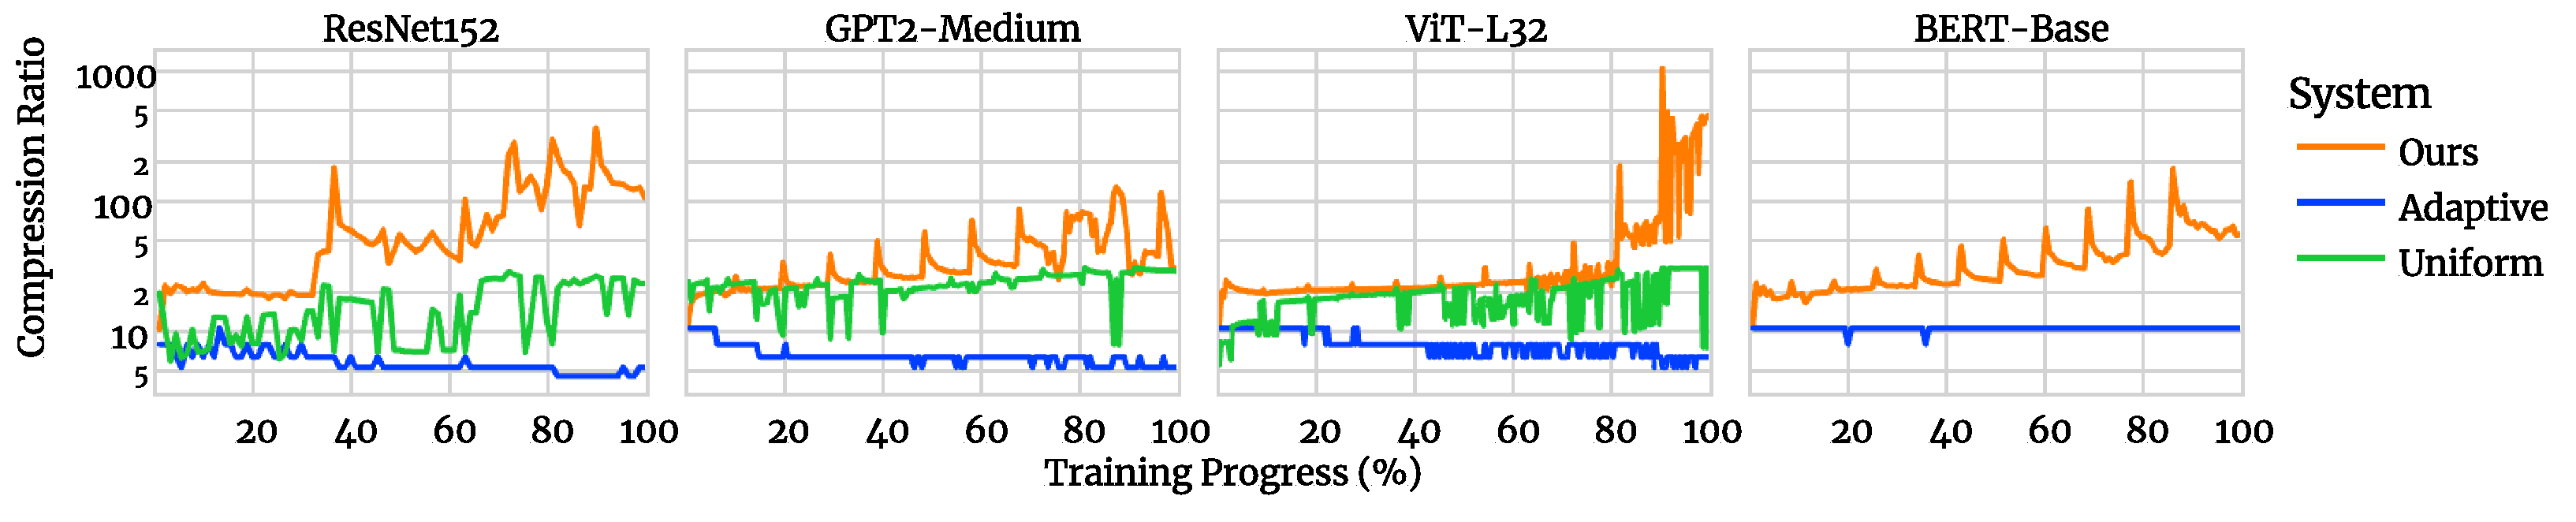
\includegraphics[width=0.99\textwidth]{figures/evaluation/cr_timeline_img.pdf}
    \caption{\small
        Compression ratio at every checkpoint during the training of various models.}
    \label{fig:cr-timeline}    
\end{figure*}



\subsection{End-to-end Evaluation: Fault-Tolerant Training}
\label{sec:eval-fr}

We conduct end-to-end training of four models under simulated failure conditions. Each experiment has 10 evenly distributed failures (every 3-8 hours of training) throughout the training duration. All models are trained using data parallelism across 8 NVIDIA A40 GPUs, with the largest models taking 3.5 calendar days (27 GPU days). 



\cref{tab:failure-recovery} compares different systems in terms of model quality, compression ratio, and runtime overhead on the failure recovery task. Overall, \sys achieves between 26-39$\times$ reduction in storage requirements across various model families, marking a 3.5-6.5$\times$ improvement over \CNR, and 1.3-3.3$\times$ improvement over \QD. This is achieved while keeping the end-to-end relative degradation below 1\%, and the overhead of our system remains less than 0.6\% of the total training time. For ViT-L32, we observe that restoring from compressed checkpoints can act as a regularization mechanism, and result in better end-to-end performance.

While \QD achieves a higher compression ratio compared to \CNR due to its delta compression ability, we find the quality of models generated by the system to be inconsistent. In particular, we see a large drop in accuracy (to 4.43\%) after 8 restores for BERT-Base training. \GOBO is omitted in this experiment as it was originally designed for post-training quantization and is significantly slower than other in-training methods (details in \S~\ref{sec:ablations}).


\cref{fig:cr-timeline} shows the change of the compression ratio throughout training, where the peaks in the compression ratio correspond to checkpoints directly following restores from the compressed state. \sys's delta encoding scheme is particularly effective during the later stages of training when model updates decelerate. \sys's peak compression performance is above 100$\times$ for all models.

\begin{table}[t]
\small
\centering
\begin{tabular}{lllll}%
\toprule
& System & Deg. \% & CR & Ovr. \%  \\
\midrule
ResNet-152 & \CNR & 0.36 & 5.71 & 0.61 \\
(Base Acc: 77.41\% )& \QD & \textbf{-0.09} & 11.82 & \textbf{0.11} \\
& \ours & 0.50 & \textbf{39.09} & 0.35 \\
\midrule
ViT L32 & \CNR & -0.21 & 7.82 & 0.96 \\
(Base Acc: 71.36\%) & \QD & 0.12 & 16.31 & \textbf{0.18} \\
& \ours & \textbf{-0.46} & \textbf{26.19} & 0.51 \\
\midrule
BERT Base & \CNR & 3.97 & 6.78 & 1.03 \\
(Base Acc: 68.49\%)& \QD & \orangecross & \orangecross & \orangecross \\
& \ours & \textbf{0.80} & \textbf{29.25} & \textbf{0.58} \\
\midrule
GPT-2 M & \CNR & \textbf{0.25} & 6.35 & 0.55 \\
(Base Loss: 2.72) & \QD & 1.10 & 22.15 & \textbf{0.10} \\
& \ours & 0.61 & \textbf{29.81} & 0.32 \\
\bottomrule
\end{tabular}
\vspace{0.5em}
\caption{\small 
    Performance of checkpoint compression systems for failure-recovery. 
    Deg. \% = Relative quality degradation, CR = Compression ratio, Overhead \% =  Runtime Overhead.
}
\label{tab:failure-recovery}
\vspace{-1.5em}
\end{table}


\cref{fig:fr-tradeoff-single} illustrates the trade-off between storage overhead and model quality under different quality thresholds ($\epsilon$) in ResNet-152 training. At $\epsilon=0.01$, we achieve 21.82$\times$ compression, with no end-to-end quality degradation. At $\epsilon=0.05$, there is a small end-to-end relative accuracy drop (0.5\%) while the compression ratio goes up to 39.09$\times$. For all thresholds, \sys demonstrates an end-to-end degradation of less than 1\% and achieves a better compression-quality tradeoff when compared to \CNR and \QD. Notably, both baselines struggle to reach high compression ratios.

Finally, \sys can withstand up to 20 restores for ResNet152, which is equivalent to a restore every 4.5 epochs, while still maintaining a relative error of 1.1\%; for reference, the error is only 0.16\% for 5 restores. 






\begin{table}[htb]
\centering
\begin{tabular}{@{\hspace{0px}} l @{\hspace{0px}} l *{5}{@{\hspace{2px}}c} @{\hspace{0px}}}
\toprule
Model & Task & Metric & Base & Adap & Uni & \ours \\
\midrule
\multirow{3}{*}{BERT--L} & & CR & - & 4.57 & 4.00 & \textbf{11.32} \\
& SST-2 & Acc & 93.2 & 92.9 & 93.0 & \textbf{93.3} \\
&  MNLI & Acc & 85.9 & \textbf{86.0} & \textbf{86.0} & 85.9 \\
& STS-B & PC & 86.1 & 87.6 & 87.8 & \textbf{88.3} \\
\midrule
\multirow{2}{*}{Pythia 1B} & & CR & - & 5.33 & 4.57 & \textbf{9.99} \\
& Alpaca & CE & 0.894 & 0.910 & \textbf{0.906} & 0.919 \\
\bottomrule
\end{tabular}
\vspace{0.5em}
\caption{\small Performance comparison on the transfer learning task.  CR = Compression ratio, Acc = Accuracy, PC = Pearson correlation, CE = Cross-entropy Loss.}
\vspace{-1em}
\label{tab:transfer-learning}
\end{table}



\subsection{End-to-end Evaluation: Transfer Learning}
\label{sec:eval-contlearn}
For the transfer learning experiments, we perform the compression process on pre-trained model checkpoints, then deploy the compressed models for downstream task fine-tuning. The checkpoints are obtained with a quality threshold $\epsilon=0.05$.  We evaluate the BERT-Base and Pythia 1B models on a suite of downstream tasks. \cref{tab:transfer-learning} shows results for all three fine-tuning tasks. We observe that for both the models, \sys can achieve compression ratios up to 11$\times$ even without delta encoding, ~2$\times$ higher compared to other systems. Notably, we find that the use of compressed checkpoints does not harm the performance of the downstream model, and we achieve performance comparable to baseline across all tasks and models.

\subsection{Microbenchmarks \& Ablation Studies}
\label{sec:ablations}


\begin{table*}[t]
\centering
\begin{tabular}{l *{3}{*{5}{c}}}
\toprule
Model & \multicolumn{12}{c}{Mean Number of Quantization Bins ($\downarrow$)}  \\
 & \multicolumn{4}{c}{0.1\% Degradation} & \multicolumn{4}{c}{1\% Degradation} & \multicolumn{4}{c}{5\% Degradation} \\
 \cmidrule{2-5}\cmidrule(lr){6-9}\cmidrule{10-13}
 & CNR+ & QD+ & GB+ & \ours & CNR+ & QD+ & GB+ & \ours & CNR+ & QD+ & GB+ & \ours  \\
\midrule
ResNet18 & 42.84 & \orangecross & \orangecross & \textbf{21.25} & 33.75 & 35.51 & 33.12 & \textbf{16.85} & 23.55 & 23.25 & 17.50 & \textbf{10.19} \\
ResNet50 & 46.36 & \orangecross & \redcross & \textbf{21.39} & 35.07 & 53.65 & 31.78 & \textbf{14.36} & 23.06 & 33.69 & 20.12 & \textbf{8.24} \\
ResNet152 & 59.32 & \orangecross & \redcross & \textbf{20.18} & 40.71 & \orangecross & \redcross & \textbf{11.92} & 26.74 & 39.36 & \redcross & \textbf{7.20} \\
MobileNet V3 Large & 65.24 & \orangecross  & \orangecross & \textbf{27.92} & 54.44 & \orangecross & \orangecross & \textbf{32.48} & 36.68 & 47.96 & 30.79 & \textbf{17.91} \\
VGG19 & 50.46 & \orangecross & \redcross & \textbf{13.06} & 31.01 & 45.36 & \redcross & \textbf{8.99} & 18.48 & 25.15 & \redcross & \textbf{6.26} \\
ViT B32 & 37.01 & \orangecross & \redcross & \textbf{19.88} & 28.37 & 38.43 & \redcross & \textbf{14.33} & 20.85 & 28.79 & \redcross & \textbf{9.75} \\
ViT L32 & 37.40 & \orangecross & \redcross & \textbf{13.31} & 32.95 & \orangecross & \redcross & \textbf{10.79} & 25.36 & 35.34 & \redcross &  \textbf{8.46} \\
BERT Base & \orangecross & \orangecross & \redcross & \textbf{54.30} & 81.45 & \orangecross & \redcross & \textbf{22.75} & 43.18 & 53.10 & \redcross & \textbf{12.74} \\
GPT-2 Medium & 106.86 & \orangecross & \redcross & \textbf{54.71} & 47.71 & 60.17 & \redcross & \textbf{16.19} & 24.60 & 31.14 & \redcross & \textbf{9.08} \\

\bottomrule
\end{tabular}
\vspace{0.5em}
\caption{
    \small One-shot compression performance under quality degradation constraints. We consider the mean number of quantization bins required to achieve the quality degradation constraint across ten evenly spaced checkpoints during training. System timeouts (30 mins for each evaluation of each configuration) are represented by \redcross, while scenarios, where no suitable configuration is found, are marked by \orangecross.}
\label{tab:one-hot-small}
\end{table*}

\begin{table}[htbp]
\centering
\begin{tabular}{@{} l *{4}{@{\hspace{6px}}c} @{}}
\toprule
Model & \multicolumn{4}{c}{Runtime in Milliseconds ($\downarrow$)} \\
 & \multicolumn{2}{c}{Quantile} & \multicolumn{2}{c}{Clustering (K=32)}  \\
\cmidrule{2-3}\cmidrule(lr){4-5}
& CuPy [\citenum{cupy}] & \ours & CuML [\citenum{cuml}] & \ours \\
\midrule
ResNet152 & 71.9 & \textbf{15.2} & 10200 & \textbf{1160} \\
ViT L32 & 364 & \textbf{80.9} & 50100 & \textbf{1140} \\
BERT Base & 155 & \textbf{33.9} & 20700 & \textbf{411} \\
GPT-2 M & 390 & \textbf{86.2} & 53400 & \textbf{819} \\
\bottomrule
\end{tabular}
\vspace{0.5em}
\caption{\small Runtime of various operations in \sys compared with off-the-shelf implementations.}
\label{tab:runtime-abalation}
\vspace{-1em}
\end{table}




\noindent\textbf{{Quality of Non-uniform Quantization.}} To evaluate different quantization algorithms, we collect ten checkpoints spaced throughout the training of different models. For each algorithm, we determine the minimum number of quantization bins needed to meet per-checkpoint thresholds of $\epsilon=0.001, 0.01, 0.05$, then calculate the mean number of bins across all checkpoints. We disable parameter pruning in our system for this experiment to allow for easier comparison. The results are presented in  \cref{tab:one-hot-small}. 

We observe that \sys consistently outperforms across all the models and quality thresholds. \GOBO, which uses a na\"ive implementation of k-means clustering algorithm for quantization, takes over 30 minutes for models with more than 30 million parameters, while \sys usually takes a few seconds. \QD fails to find valid quantization configurations for strict quality thresholds. Among baselines, only \CNR manages to constantly find quantization configurations that satisfy the quality thresholds. However, it requires a 2-4$\times$ higher number of quantization bins to achieve the same quality as \sys due to their use of uniform quantization.


\noindent\textbf{{Quantization Runtime.}} \cref{tab:runtime-abalation} reports the runtime of two key operations in our quantization algorithm: computing qualities for pruning and protection, and the \kmeans clustering for quantization. We implement our approach in Pytorch with support for both CPU and GPU execution. We compare the performance of our implementation against off-the-shelf GPU-enabled implementations for quantile estimation in CuPy and \kmeans clustering in CuML respectively. Our quantile estimation algorithm achieves 3-4$\times$ higher performance compared to CuPy, while we note a speed-up of up to 65$\times$ in quantile computation. 







\begin{figure}
    \centering
    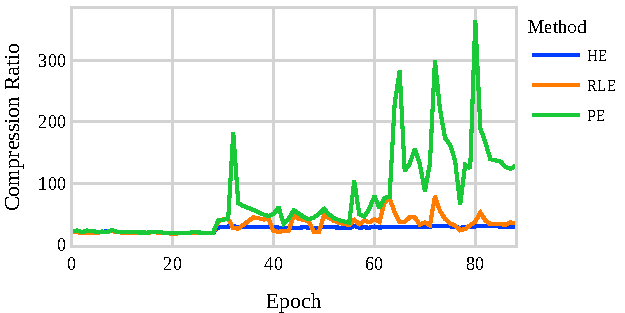
\includegraphics[width=0.9\linewidth]{figures/evaluation/delta_ablation_img.pdf}
    \caption{
    \small 
        Parameter rearrangement significantly improves the performance of delta encoding schemes (ResNet-152).
        HE = Huffman Encoding, RLE = Run Length Encoding + Huffman Encoding, PE = Parameter Rearrangement-based Encoding.}
    \label{fig:delta-abalation}
    \vspace{-1em}
\end{figure}


\noindent\textbf{Parameter Rearrangement-based Delta Encoding.} 
The key optimization in \sys's delta encoding scheme is parameter rearrangement, which enables it to decrease the entropy in each compressed chunk. 
To assess the contribution of this optimization, we compare three variants of our delta encoding scheme: the Huffman encoding variant used in \QD (HE), run-length plus Huffman encoding (RLE), and parameter rearrangement-based delta encoding (PE) on the ResNet-152 training job. The results are illustrated in \cref{fig:delta-abalation}. With parameter rearrangement, we achieve much higher compression in the later phase of training. Notably, we obtain a maximum compression ratio of 366 with rearrangement compared to 79 with RLE and 30 with HE. This translates to overall lower storage overhead. The Huffman and run-length encoding-based schemes only achieve overall storage overhead reduction of 25$\times$ and 28$\times$ respectively, as opposed to 39$\times$ with parameter rearrangement.

